\documentclass[12pt]{article}
\usepackage[utf8]{inputenc}
\usepackage{amsmath,amssymb}
\usepackage{unicode-math}
\usepackage[T2A]{fontenc}
\usepackage[russian]{babel}
\usepackage{graphicx}
\usepackage{subfigure}
\usepackage{subcaption}
\usepackage{url}


\DeclareGraphicsExtensions{.pdf,.png,.jpg}
\usepackage{hyperref}
\usepackage{wrapfig}
\usepackage[left=20mm, top=20mm, right=10mm, bottom=20mm]{geometry}

\usepackage{amsmath} 
\usepackage{amsfonts} 
\usepackage{amssymb} 
\usepackage{wasysym} 
\usepackage{fancyhdr}

\pagestyle{fancy}
\fancyhf{}
\lhead{Семинар 8. Эффект Зеемана. Правила отбора}
\rhead{\textit{Клименок К.Л., МФТИ 2020}}
\rfoot{\thepage}



\begin{document} 
\title{\textbf{Семинар 8. Эффект Зеемана. Правила отбора}}
\author{\textbf{Клименок Кирилл Леонидович}}
\date{30.09.2020}
\maketitle
\section{Теоретическая часть}
На данный момент мы с вами разобрались с устройством уровней энергии в разных сложных атомах, поняли, что такое спин и даже научились (надеюсь) писать термы различных энергетических состояний атома. Пришло время перейти к переходам между различными уровнями и поведении этих уровней энергии во внешнем магнитном поле.\\
Мне кажется, что уже становится понятно, если мы включим внешнее магнитное поле в выделенном направлении, то из-за проекции полного магнитного момента атома на это направление каждый уровень начнет расщепляться по энергиям, это приведет к еще большей сложности в строении уровней (эффект Зеемана) и к куче разных переходов между ними. А вот тут оказывается, что все не совсем однозначно. Некоторые переходы оказываются невозможны в силу правил отбора. Давайте про них и поговорим перед эффектом Зеемана
\subsection{Правила отбора}
\paragraph{Четность} Начнем с понятия четности и ее оператора. Вы конечно знаете про правые и левые тройки векторов в трехмерном пространстве, и что одна из них является зеркальным отражением другой. Можно ли тогда ввести  оператор инверсии, который бы зеркально транслировал наше обычное пространство в зеркальное. Да, разумеется, это делается очень легко, такой оператор называется оператором четности: $\hat{\mathfrak{p}}$ (я буду использовать готическое начертание, чтобы не путать с импульсом) все что он делает -- это изменение вектора координаты $\textbf{r} \rightarrow -\textbf{r}$. Давайте найдем собственные значения этого оператора, просто применив его 2 раза подряд:
\begin{gather*}
\hat{\mathfrak{p}}\psi(r) = \mathfrak{p} \psi(r)=\psi(-r)\\
\hat{\mathfrak{p}^2}\psi(r) = \mathfrak{p}^2 \psi(r) = \psi(r)\\
\mathfrak{p} = \pm 1
\end{gather*}
То есть собственные значения это или 1 или -1, а собственные функции это любые четные или не четные волновые функции. \\
Но в физике мы встречались не только с нормальными (истинными) векторами, которые при изменении четности меняют направление, но и другими векторами, которые называются аксиальными или псевдовекторами (например момент импульса или магнитный момент). Этот вектор не меняется с преобразованием инверсии. Почему это так, можно проследить на рисунке \ref{fig:sem_08_pic_1}
\begin{figure}[h]
    \centering
    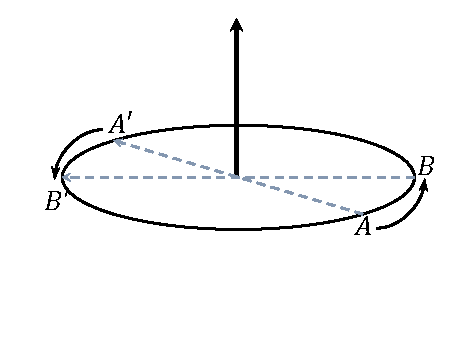
\includegraphics[width=0.6\textwidth,height=\textheight,keepaspectratio]{Seminar_08/pics/pic_01.pdf}
    \caption{Постоянство аксиального вектора при инверсии}
    \label{fig:sem_08_pic_1}
\end{figure}
Теперь скажем про знакомые нам системы, где появляется момент импульса $l$, например атом. Что тогда будет с четностью? Ответ можно получить строго, подставив известные нам решения уравнения Шредингера для случая сферически симметричного случая, это я опущу и скажу, что для такой системы $\mathfrak{p} = (-1)^l$. Если же система состоит из нескольких частей, то помимо простого произведения четности каждой из компонент этой системы, нужно учесть еще четность из относительного движения: $\mathfrak{p} = \mathfrak{p}_A\cdot\mathfrak{p}_B\cdot (-1)^{(l_A+l_B)}$. Более того, для всех типов взаимодействия, кроме слабого, работает закон сохранения четности. 
\paragraph{Золотое правило Ферми. Вероятности переходов}
Рассмотрим вот такую задачу:
\begin{equation*}
    \begin{cases}
    \hat{H_0}\psi_i=E_i\psi_i\\
    \hat{H}=\hat{H_0}+\hat{A}\xi \cos{\omega t}
    \end{cases}
\end{equation*}
Пусть у нас есть задача на поиск стационарных решений для известного оператора Гамильтона с индексом 0 и все уровни энергии $E_i$ мы знаем, тогда теперь добавим переменное по времени слабое по сравнению с остальным воздействие на систему. Это будет наше переменное поле, с которым наша система взаимодействует. Под действие такого вот воздействия система может поменять свое состояние с вероятностью:
\begin{equation*}
    \rho_{ij} \sim \left| \int \psi^*_i\hat{A}\xi\psi_j dV\right|^2 \delta (E_i-E_j \pm \hbar \omega)
\end{equation*}
Это и есть золотое правило Ферми. Дельта-функция здесь просто говорит нам о законе сохранения энергии и подборе частоты так, чтобы расстояние между известными уровнями точно соблюдалось, а вот с интегралом надо бы разобраться подробнее. Во-первых что же такое оператор $\hat{A}$ и какой смысл он в себе несет? Это оператор физической величины системы, который обеспечивает связь с переменным воздействием. Если говорить об атоме, то это может быть, например, оператор дипольного момента атома, как электрического, так и магнитного или просто заряд атома или что-то более сложное. А что это за состояния и что означает этот интеграл. Мы знаем, что i и j состояния, это собственные состояния системы и они являются независимыми. То есть получается, что наш оператор $\hat{A}$ должен <<перепутать>> наши состояния, иначе перехода не произойдет. Более того, мы можем переставить i и j местами и вероятность от этого никак не измениться. То есть неважно переход идет снизу вверх или сверху вниз.
\paragraph{Мультипольное разложение. E и M фотоны}
Теперь давайте посмотрим и запишем более подробно, какие у нас могут быть физические величины у разных систем, который взаимодействует с электромагнитным полем. Начнем с электрической составляющей. Первое, что приходит на ум, это просто записать положение каждого конкретного заряда в системе и закончить с этим. Это может быть совершенно нерационально, особенно, если мы говорим о сложном атоме, где десятки протонов и электронов, которые как-то живут вокруг ядра. Более того, не факт, что наше поле, которое взаимодействует с атомом существенно меняется с положением внутри атома. Поэтому мы можем воспользоваться трюком, который носит название <<мультипольное разложение>>. В чем его суть? Давайте объединим все эти зарядики, которые сидят в атоме и представим их как одни -- простая сумма зарядов (скаляр $q = \sum q_i$). Это первый член такого разложения. Обычно нам везет и атом нейтрален, поэтому суммарный заряд равен 0. Но ведь атом с полем взаимодействует! Тогда можем заменить нашу систему зарядов диполем с известным положением плюса и минуса (вектор $\textbf{d} = \sum q_i \textbf{r}_i$). А вот такая штука совершенно не обязательно равна нулю. Если нам этого не хватает можем пойти дальше и сделать из зарядов квадруполь (тензор второго ранга, или проще матрица $Q_{\alpha\beta} = \sum q_i(3r_{i\alpha}r_{i\beta}-r^2\delta_{\alpha\beta}) $, см. \ref{fig:sem_08_quad}) и так далее. Тогда суммарная энергия взаимодействия с таким вот разложением:
\begin{equation*}
    \varepsilon = q\phi - (\textbf{d}\cdot\textbf{ E}) - \dfrac{1}{2}\sum Q_{\alpha\beta}\dfrac{\partial E_{\alpha}}{\partial r_{\beta}}+ \dots
\end{equation*}

\begin{figure}[h]
    \centering
    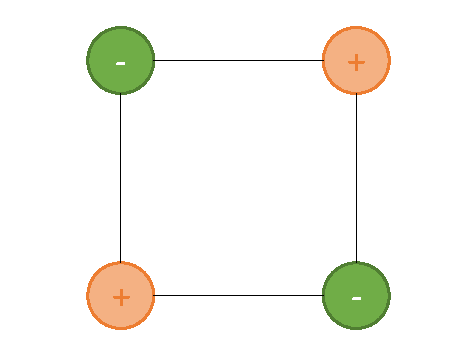
\includegraphics[width=0.4\textwidth,height=\textheight,keepaspectratio]{Seminar_08/pics/pic_02.pdf}
    \caption{Квадруполь}
    \label{fig:sem_08_quad}
\end{figure}
Для магнитного поля обычно достаточно рассмотреть магнитный момент и все, но тоже можно извратиться и двинуться в сторону квадруполей.\\
А теперь наконец давайте попытаемся сформулировать правила отбора по четности. Для этого еще раз смотрим на вероятность перехода между состояниями из золотого правила Ферми на примере электрического дипольного момента:
\begin{equation*}
    \rho_{ij} \sim \left| \int \psi^*_i\hat{d}\psi_j dV\right|^2
\end{equation*}
Электрический дипольный момент это истинный вектор и при преобразовании инверсии его знак меняется на противоположенный, но ведь инверсия это просто выбор правой или левой системы координат, а природа не знает различий между ними и переход, если он возможен, будет в любой из систем. Тогда смотрим на этот интеграл и видим, что если состояния обладают одинаковой четностью к инверсии, то под интегралом стоит нечетная функция и такой интеграл равен нулю. То есть для дипольного электрического перехода необходимо изменение четности состояния. Мы уже показали, что четность определяется как $(-1)^l$, что означает что такие переходы разрешены между S и P состояниями, но запрещены между например S и S состояниями. Аналогично это работает и с другими электрическими компонентами мультипольного разложения. Все такие фотоны называются электрическими, или как обычно пишут $Ej$ фотоны, где $j=1$ -- диполь, $j=2$ -- квадруполь и т.д. Для них пространственная четность $(-1)^j$

Теперь рассмотрим в качестве <<запутывающего>> оператора оператор магнитного момента. Опять смотрим на золотое правило Ферми и видим: магнитный момент -- аксиальный вектор, не меняется при инверсии, значит чтобы этот интеграл не занулился, нам нужна одинаковая пространственная четность наших состояний. Это означает что магнитные фотоны появляются при переходах между S и S или S и D состояниями. И по аналогии такие фотоны обозначаются $Mj$, где $j$ также показывает <<-польность>> фотона. Для них пространственная четность $(-1)^{j+1}$

Теперь пару слов о вероятности излучения тех или иных фотонов. Вопрос вполне ожидаемый, а каких больше? Давайте ограничимся только случаем диполей. Вспомним из электричества, что интенсивности излучаемые диполем пропорциональны квадрату второй производной от дипольного момента:
\begin{gather*}
    I_e \sim \ddot{p_e}^2 \sim \left(\ddot{\sum{e_i r_i}} \right)^2\\
    I_{\mu} \sim \ddot{p_{\mu}}^2\sim \left(\ddot{\dfrac{1}{2c}\sum{e_i [r_i v_i]}} \right)^2\\
\end{gather*}
Тут сразу же становится видно, что $ I_{\mu} \sim  I_{e} \left(\dfrac{v}{c} \right)^2\approx I_e \cdot 10^{-7}$ то есть электрических фотонов много больше. Аналогично можно посмотреть на более страшные формулы для квадрупольного излучения и получить похожие результаты.

\paragraph{Спин фотона. Правила отбора для E1-фотонов.} Кажется, куда уж дальше?! Но на самом деле, самая забавная штука ждет нас именно здесь. Оказывается у фотонов есть спин. Вот тут точно у последних из вас окончательно вскипел мозг. Спин это же собственный магнитный момент (и связанный с ним момент импульса) для частицы (так по крайней мере было у электрона), но говорить об этом мы можем только, если мы сядем в систему отсчета частицы, где она покоится, а фотон движется со скоростью света в любой системе.  Совсем грустно стало? Это нормально. Но вот тут нам на помощь придет оптика прошлого семестра. Помните, мы говорили о разных поляризациях электромагнитных волны. В том числе среди прочих была и круговая. Вот к спину фотона надо относится именно как к круговой поляризации, только не волны в целом, а конкретного фотона. Так а какие значения он может принимать? Во-первых, для фотонов работает принцип суперпозиции и нет принципа Паули, значит спин целый или 0. Во-вторых, есть эффект Садовского, когда мы светим поляризованным по кругу светом на мишень и она начинает крутиться, то есть момент импульса фотоны все-таки переносят. Окончательно спин фотона целый и не нулевой. При этом спин однозначно связан с <<-польностью>> фотона, т.е. у дипольных фотонов он равен 1, для квадрупольных 2 и т.д.

Ну и теперь, поскольку самым распространенным в природе являются $E1$- фотоны (дипольные электрические), то для них мы и запишем правила отбора, которые по своей сути являются законами сохранения момента импульса и четности:
\begin{itemize}
    \item $\Delta S =0$. Действительно, ведь фотон электрические, а изменение спина связано с магнитным моментом.
    \item $\Delta J = \pm 1, 0$. Ноль возможен, если проекция на выделенное направление сохраняется, а фотон уносит полный момент в другой проекции
    \item $\Delta L = \pm 1, 0$. По сути закон сохранения четности
\end{itemize}

\subsection{Эффект Зеемана}
А вот теперь можно поговорить и об атоме в магнитном поле и об эффекте Зеемана, который описывает расщепление уровней энергии атома в этом внешнем магнитном поле.

Что мы уже знаем/помним из прошлой недели? Есть тонкое расщепление уровней, связанное со спин орбитальным взаимодействием, которое легко объясняется, если мы <<пересаживаемся>> электрон, ядро начинает вращаться вокруг него и спин электрона начинает с магнитным полем этого ядра взаимодействовать. Теперь же у нас есть еще и внешнее магнитное поле и мы должны рассмотреть случаи, когда это внешнее поле много меньше поля от этого <<движущегося>> ядра, то есть спин-орбитальное взаимодействие превалирует (слабое поле, $\mu B_{ext} \ll E_{LS}$) и альтернативный случай, когда на спин-орбитальное взаимодействие мы можем забить (сильное поле, $\mu B_{ext} \gg E_{LS}$).

\paragraph{Слабое поле} Тут у нас определяющим является спин-орбитальное взаимодействие, а магнитный момент атома будет определяться через полный механический момент атома и его g-фактор: $\mu_J = -g\mu_{\text{Б}}J$ и тогда энергия во внешнем поле будет определяться проекцией полного момента на внешнее поле: $U_B = -(\mu_J B) = g\mu_{\text{Б}}m_JB$, а проекции могут быть: $m_J = \pm J, \pm (J-1), \dots$. Пример для стандартного дуплета натрия представлен на \ref{fig:sem_08_weak_zeeman}.

\begin{figure}[h]
    \centering
    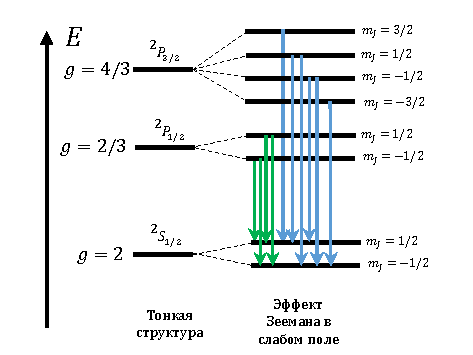
\includegraphics[width=0.7\textwidth,height=\textheight,keepaspectratio]{Seminar_08/pics/pic_03.pdf}
    \caption{Эффект Зеемана в слабом магнитном поле}
    \label{fig:sem_08_weak_zeeman}
\end{figure}

\paragraph{Сильное поле} Тут у нас спин-орбитальное взаимодействие вообще не играет роли и никакого тонкого расщепления нет, а магнитный момент атома будет определяться независимо через механические и спиновый моменты $L$ и $S$. Я напомню, что вклад спиного момента в магнитный момент в 2 раза больше, чем у механического и это надо будет учесть. Опять рассматриваем переход между $^2P$ и $^2S$. Расщепление уровней состояний представлены в таблице.


\begin{figure}[h]
    \centering
    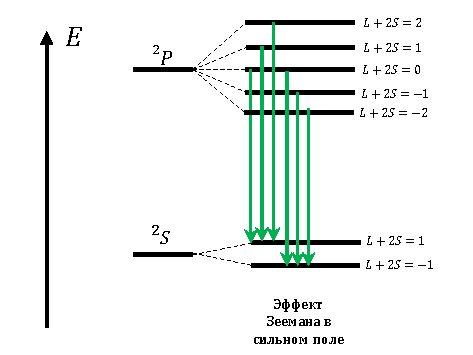
\includegraphics[width=0.7\textwidth,height=\textheight,keepaspectratio]{Seminar_08/pics/pic_04.pdf}
    \caption{Эффект Зеемана в сильном магнитном поле}
    \label{fig:sem_08_strong_zeeman}
\end{figure}


\begin{table}[]
\centering
\begin{tabular}{|l|l|l|}
\hline
\multicolumn{3}{|c|}{$^2P$}                                                                 \\ \hline
\multicolumn{1}{|c|}{$L_z$} & \multicolumn{1}{c|}{$S_z$} & \multicolumn{1}{c|}{$L_z+2S_z$} \\ \hline
1                          & 1/2                       & 2                               \\ \hline
1                          & -1/2                      & 0                               \\ \hline
0                          & 1/2                       & 1                               \\ \hline
0                          & -1/2                      & -1                              \\ \hline
-1                         & 1/2                       & 0                               \\ \hline
-1                         & -1/2                      & -2                              \\ \hline
\multicolumn{3}{|c|}{$^2S$}                                                                 \\ \hline
0                          & 1/2                       & 1                               \\ \hline
0                          & -1/2                      & -1                              \\ \hline
\end{tabular}
\caption{Расщепление уровней для эффекта Зеемана в сильном поле}
\end{table}

\subsection{ЭПР и ЯМР}
Тут особенно много я рассказывать не буду, а просто расскажу классическую интерпретацию этих резонансный явлений. У нас есть спин (в случае электронного парамагнитного резонанса у электрона, в случае ядерного -- у ядра), у нас есть внешнее постоянное магнитное поле. Спин может быть направлен по или против этого поля, в зависимости от этого энергия у такого спина будет разной. Но под действием внешнего переменного поля мы можем заставить спин поворачиваться. Это соответствует обычному переходу в двухуровневой системе. В качестве альтернативы, можно сказать, что это переход соответствует $M1$ фотонам.

Основная формула этого эффекта:
\begin{equation*}
    \hbar \omega_0 = g\mu B
\end{equation*}




\section{Практическая часть}
\subsection{Задача 6.21}
\label{task_6.21}
\paragraph{Условие} При переходе $P \rightarrow S$ возбужденного состояния атома в основное испускается дублет $\lambda_1 = 455.1$ нм и $\lambda_2 = 458.9$ нм. Какие линии, соответствующие переходу $^2S_{1/2} \rightarrow ^2P_{3/2}$, наблюдаться в спектре поглощения газа, состоящего из таких атомов, при наложении магнитного поля 50 кГс при температуре $T=0.5$ K?
\paragraph{Решение}
Первое, с чем определимся это то какой это эффект Зеемана -- в сильном или слабом поле? Считаем характерные энергии спин-орбитального взаимодействия и взаимодействия с магнитным полем:
\begin{gather*}
    U_{LS} = \dfrac{hc}{\lambda^2}\Delta \lambda = 2\cdot 10^{-2} \text{ эВ}\\
    U_B = \mu B = 3\cdot 10^{-4} \text{ эВ}\\
    kT = 4\cdot 10^{-5} \text{ эВ}\\
\end{gather*}
То есть это слабое поле, при этом все атомы сидят в нижнем положении по энергии, а сама задача стоит о поглощении а не испускании. А дальше смотрим на известную нам из теории структуру линий для этого эффекта из теории и просто записываем разницы энергий:
\begin{gather*}
    E_B=\mu B(g_1m_{j1} - g_21m_{j2})\\
    E_B = \mu B 
    \begin{cases}
    4/3 \cdot 1/2 - 2\cdot(-1/2) = 5/3\\
    4/3 \cdot (-1/2) - 2\cdot(-1/2) = 1/3\\
    4/3 \cdot (-3/2) - 2\cdot(-1/2) = -1\\
    \end{cases}
\end{gather*}
аналогично можно посчитать энергии переходов из состояния с полным моментом 1/2, но в силу маленькой температуры, заселенностью этого состояния можно пренебречь.


\subsection{Задача T4}
\label{task_t4}
\paragraph{Условие}
Ион меди $Cu^{2+}$, входящий в состав многих магнитных солей, имеет электронную конфигурацию внешней незаполненной оболочки $3d^9$. 1) Определить квантовые числа свободного иона меди $Cu^{2+}$; записать его спектроскопический символ и вычислить g-фактор. 2) В ионных кристаллах магнитный ион взаимодействует с электрическим полем своих соседей, поэтому его более нельзя считать свободным и формула Ланде становится неприменимой. В соли $CuGeO_3$ (магнитным моментом в этом соединении обладает только ион $Cu^{2+}$) в одной из ориентаций магнитного поля относительно кристалла резонансное поглощение наблюдается на частоте $\nu = 36.5$ ГГц в поле $H = 11.48$ кЭ. Определить по этим данным эффективный g-фактор иона меди в этом кристалле.
\paragraph{Решение}
На самом деле задачка очень простая, нужно лишь потренироваться переписывать электронные конфигурации в термы и определять основные параметры атома. Начнем как раз  с этого. у нс есть d-орбиталь, на ней момент $L=2$, но из 10 возможных электронов заполнено 9, значит все кроме одного спарены и спиновый момент $S=1/2$. Тогда полный момент $J=L+S = 5/2$. Для нахождения g-фактора надо просто воспользоваться формулой из прошлого семинара и получается $g=6/5$.

Для второй части надо воспользоваться основной формулой для эффекта ЯМР/ЭПР:
\begin{gather*}
    h\nu = g\mu B\Rightarrow g = \dfrac{h\nu}{\mu B} = 2.27
\end{gather*}


\subsection{Комментарии к задачам из задания}
\paragraph{Задача 6.21} Решена 
\paragraph{Задача 6.34} Повторяет 6.21. Так же использовать схему из теоретической части
\paragraph{Задача 6.58} Тут нужно найти разность населенности 2 уровней энергии, как для обычной двухуровневой системы с распределением Больцмана.
\paragraph{Задача T3} Определить изменение четности и изменение момента 2 состояний, по этим изменениям определить фотон. Время жизни обратно пропорционально вероятности излучения, поэтому из данных задачи надо собрать что-то похожее на безразмерный $(v/c)^2$ 
\paragraph{Задача T4} Решена
\paragraph{Задача 1.57} Опять двухуровневая система для которой надо найти среднюю разность заселенностей, которая и будет пропорциональная вероятности поглощения
\paragraph{Задача 1.59} Тут нужно записать баланс того сколько излучилось с верхнего уровня к тому сколько поглотилось и ушло из резонатора

\end{document}
